\documentclass[../../main.tex]{subfiles}

\lstset{basicstyle=\small,
      showstringspaces=false,
      commentstyle=\color{black},
      keywordstyle=\color{blue}
    }
\emergencystretch 1em  % F"ur TeX <3.0 auskommentieren!
\graphicspath{{images/Signalerkennung/}{../../images/Signalerkennung/}}


\begin{document}
\subsection{Signalerkennung}
    In der Aufgabenstellung wird gefordert, dass der Schnellzug während der Bewältigung der Strecke ein Signal mit aufgedruckter Nummer erkennt wird. Die Nummer ist auf einer 3x3cm Tafel mit weissem Hintergrund, schwarz aufgedruckt. Die Aufgabe Signalerkennung wird in zwei Teilaufgaben unterteilt:
    \begin{itemize}
        \item Erkennung der Signalisation mit Tafel
        \item Erkennung der aufgedruckten Nummer
    \end{itemize}
    Wie bereits in der Übersicht beschrieben, wird im Gesamtkonzept zwei Kameras verwendet. Eine Kamera wird zur Erkennung der Schienenrichtung verwendet. Die zweite Kamera wird nun für die Signalerkennung eingesetzt. Der Raspberry PI 3+, welcher als Hauptrecheneinheit geplant ist, verfügt nur über einen CSI- Anschluss (Camera Serial Interface). Für die Signalerkennung wird auf einen weiteren kleineren Raspberry PI 3 Model A+ gesetzt. Dieser verfügt wie der Raspberry PI 3+ einen vollwertigen CSI- Anschluss und kann somit die zweite Kamera bedienen. Dies führt auch dazu, dass der Raspberry PI 3+ zusätzlich entlastet werden kann.\\

    \textbf{Architektur}\\
    Die Signalerkennung in zwei Teilaufgaben zu trennen hat noch einen weiteren vorteil. Die beiden Teilaufgaben werden auf beide Raspberry PIs verteilt. Der Raspberry PI 3 Model A+ ist für die Bilderaufnahme Verarbeitung und für die Signalerkennung mit Tafel zuständig. Der Raspberry PI 3+ übernimmt dann die Erkennung der aufgedruckten Nummer auf der Tafel. So kann die Ressourcen des Raspberry PI 3+ gezielter eingesetzt werden.

    \begin{figure}[H] %Architektur
        \centering
        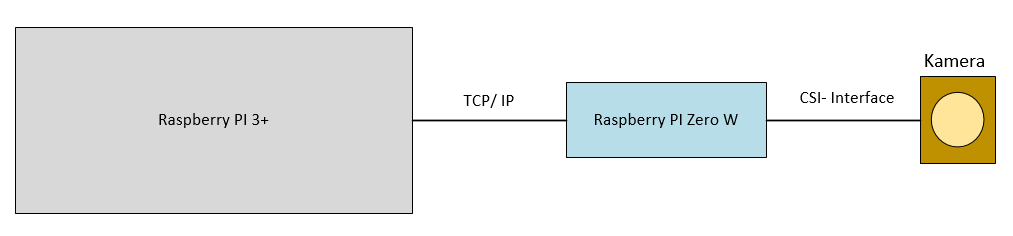
\includegraphics[width=0.9\textwidth]{Architektur.png}
        \caption{Architektur Hardware Signalerkennung}
        \label{fig:architektur_hardware_signalerkennung}
    \end{figure}

    Für die Nummererkennung auf der Tafel Machine- Learning Algorithmus verwendet. Damit die Trainingsdaten des Models eingelesen werden können und somit ausführbar wird, braucht es eine gewisse grösse des Arbeitsspeichers. Der Arbeitsspeicher des Raspberry PI 3 Model A+ (512Mb) reicht dafür nicht aus. Der Raspberry PI 3+ verfügt über mehr speicher (1Gb) und kann somit den Algorithmus bearbeiten. Für die Kameraufnahmen und die Bearbeitung der Bilder und schlussendlich die Konturenerkennung der Signalisation ist der Raspberry PI 3 Model A+  gut geeignet.
    \pagebreak

    \textbf{Software Tafelerkennung}\\
    Für die Erkennung der Tafel wird auf das Framework OpenCV gesetzt. OpenCV hat sich als Standartframework im Bereich der Echtzeitbildverarbeitung. Weiter zeichnet sich OpenCV in seiner Effizienz und seiner breiten Community, welche im Internet mit vielen Tutorial zu hilfe stehen. In der Abbildung \ref{fig:ablauf_tafelerkennung} ist der Abblauf der Tafelerkennung und in der Tabelle \ref{tab:OpenCV_Funktionen_Tafelerkennung} die jeweilige Funktion beschrieben.



    \begin{figure}[H] %Vision Ablauf
        \centering
        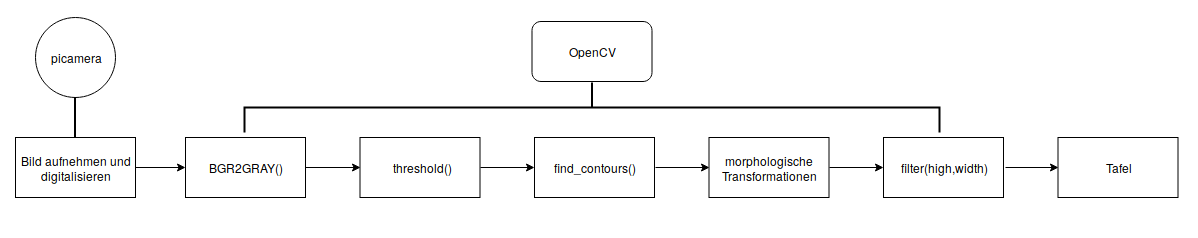
\includegraphics[width=1\textwidth]{Ablauf_Tafelerkennung.png}
        \caption{Ablauf Erkennung der Tafelerkennung}
        \label{fig:ablauf_tafelerkennung}
    \end{figure}

    \begin{table}[H]
        \begin{flushleft}
            \begin{tabular}{ | p{3cm} | p{10.5cm} |}
                \hline
                \textbf{Funktion}  & \textbf{Beschreibung} \\\hline
                Bild aufnehmen und digitalisieren & Die Umgebung wird mittels der Raspberry PI Kamera und der Bibliothek picamera aufgenommen und dem OpenCV übergeben \\\hline
                BGR2GRAY & Die Farbinformation vom Bild werden nicht benötigt und deshalb entfernt (Effizienz) \\ \hline
                threashold & Für die Konturenerkennung braucht es nur die Schattierungen des Bildes. Aus diesem Grund wird ein Threashold auf das Bild gelegt damit ein Binery- Picture generiert werden kann. \\ \hline
                find-contours & Nun wird die OpenCV Funktion find-contours angewendet. Dabei werden benachbarte Schwarz oder Weiss Pixel miteinander zusammengefügt bis eine Kontur entstehen kann. \\ \hline
                morphologische Transformationen & Hier wird das Bild mittels morphologische Transformationen nachbearbeitet \\ \hline
                filter & Die erkannten Konturen werden gefiltert nach der Grösse und Form der Tafel. \\ \hline
                Tafel & Nun ist das Bild mit der Tafel erkannt worden und wird zur Nummererkennung vorbereitet. \\ \hline
            \end{tabular}
        \end{flushleft}
        \caption{Beschreibung der OpenCV Funktionen}
        \label{tab:OpenCV_Funktionen_Tafelerkennung}
     \end{table}

     In der Abbildung \ref{fig:tafelerkennung} links sieht man die erkannte Position der Nummer auf der Tafel. Rechts sieht man die gleiche Aufnahme nach der Filterung. Dieses Bild wird nun auf die Grösse des rechten Erkannten Rechteckes zugeschnitten und dem Raspberry PI 3+ zur Nummererkennung übergeben.\\

     \textbf{Konfiguration Raspberry PI Kamera}\\
     Eine weitere Schwierigkeit bei der Nummererkennung ist die Aufnahme mittels Kamera. Bei hohen Geschwindigkeiten neigt das Bild dazu unscharf zu werden. Dies liegt daran, dass die Verschlusszeit der Kamera zu lange ist. Mit der Raspberry PI Kamera und der Schnittstelle piCamera können viele Parameter eingestellt werden. Hier liegt der Schlüssel zur Behebung von unscharfen Bildern. Wenn Parameter wie Belichtungszeit, Helligkeit, Sättigung und Weissabgleich fest eingestellt werden, können in erster Linie reproduzierbare Bilder aufgenommen werden und die Belichtungszeit kann auf ein Minimum gesetzt werden. Wenn die Belichtungszeit kürzer gesetzt wird, ist das Ergebnis aber dunklere Bilder. Mit digitaler Aufhellung oder sogar mit externer Beleuchtung kann aber diesen Effekt entgegengesetzt werden. 

     \begin{figure}[H] %Vision Ablauf
        \centering
        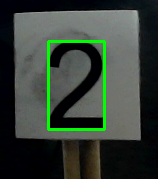
\includegraphics[width=0.2\textwidth]{number_location.png}
        \hspace{1cm}
        
\includegraphics[width=0.17\textwidth]{number_thres.png}
        \hspace{1cm}
        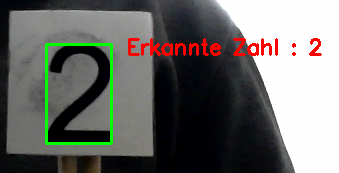
\includegraphics[width=0.4\textwidth]{number_reco.png}
        \caption{Nummerposition- und Nummererkennung}
        \label{fig:tafelerkennung}
    \end{figure}

    \textbf{Software Nummererkennung}\\
    Damit nun die Nummer auf der Tafel erkannt werden kann, wird ein Machine- Learning Algorithmus verwendet. Dafür wird die high-level API Keras verwendet. Als Backend kommt Tensorflow zum Einsatz. Als Trainingsdatabase kommt die frei Verfügbare MNIST- Database zu Einsatz. Die MNIST- Datenbank verfügt über 60'000 Zahlen in Handschrift. In Tabelle XX ist die Zusammenfassung der Tensorflowbackend bezüglich dem ausgewählten Keras Model. In den ersten Tests hat die Erkennung gut funktioniert auch auf dem Raspberry PI. Probleme sind in erster Linie mit der Nummer "1" aufgetaucht. Die MNIST Datenbank verfügt nur über die amerikanisch geschriebene "1". Die "1" in Arial wird dadurch nicht erkannt. Sobald in PREN2 die Schriftart der Zahlen bekannt gegeben wird, muss eventuell einen eigenen Trainingsdatensatz erstellt werden oder auf einen anderen Datensatz wie zum Beispiel von UCI Machine Learning Repository. 
    \begin{table}[H]
            \begin{center}
                \begin{tabular}{ | l | l | p{3cm} |}
                \hline
                \textbf{Layer(type)}  & \textbf{Output Shape} & \textbf{Param \#}\\\hline
                conv2d\_1 (Conv2D) & (None, 26, 26, 32) & 320 \\\hline
                conv2d\_2 (Conv2D) & (None, 24, 24, 64) & 18496 \\ \hline
                max\_pooling2d\_1 (MaxPooling2) & (None, 12, 12, 64) & 0\\ \hline
                dropout\_1 (Dropout) & (None, 12, 12, 64) & 0 \\ \hline
                flatten\_1 (Flatten) & (None, 9216) & 0 \\ \hline
                dense\_1 (Dense) & (None, 128) & 1179776 \\ \hline
                dropout\_2 (Dropout)  & (None, 128) & 0 \\ \hline
                dense\_2 (Dense)  & (None, 10) & 1290 \\ \hline
                \end{tabular}
            \end{center}
            \caption{Auflistung aller Testklassen mit jeweiliger Testarten}
            \label{tab:Testklassen}
        \end{table}
\end{document}